\subsubsection{Kpetene-Gruppe}\label{sec:KPT-Gr}

\todo[inline]{
Zur Frage vom KPT eine vollwertige Stilgruppe ist:
- siehe auch Wotzka 1995: 185 Angaben zum 'Status' der Bolombi-Gruppe \& 202 Mpokioko-Gruppe!
}

Die Kpetene-Gruppe fasst eine geringe Anzahl von rouletteverzierten Gefäßen und Gefäßfragmenten zusammen, die am oberen Ubangi gefunden wurden (Abb.~\ref{fig:KPT_Verbreitung}). Lediglich acht GE konnten der Stilgruppe zugewiesen werden, wobei in lediglich drei Fällen eine Ansprache zweifelsfrei möglich war.


\paragraph{Technologische Merkmale}
$\;$ \\
Die wenigen Stücke der Kpetene-Gruppe zeichnen sich durch einen Scherben aus, der größere Anteile nichtplastischer Partikel der Korngrößen \textit{coarse} und \textit{very coarse} enthält. Regelhaft handelt es sich um Quarzsand sowie Glimmer und ausgebrannte Organik. In zwei Fällen konnten auch geringe Anteile Schamott in den Scherben beobachtete werden. Die genutzten Tone sind häufig rotbrennend (50\,\%), nur eine GE deutet die Nutzung weißbrennender Tone an. Die Oberflächen der Scherben sind häufig geglättet (57\,\%).

\begin{figure*}[tb]
	\centering
	\begin{subfigure}[b]{.49\textwidth}
		\centering
		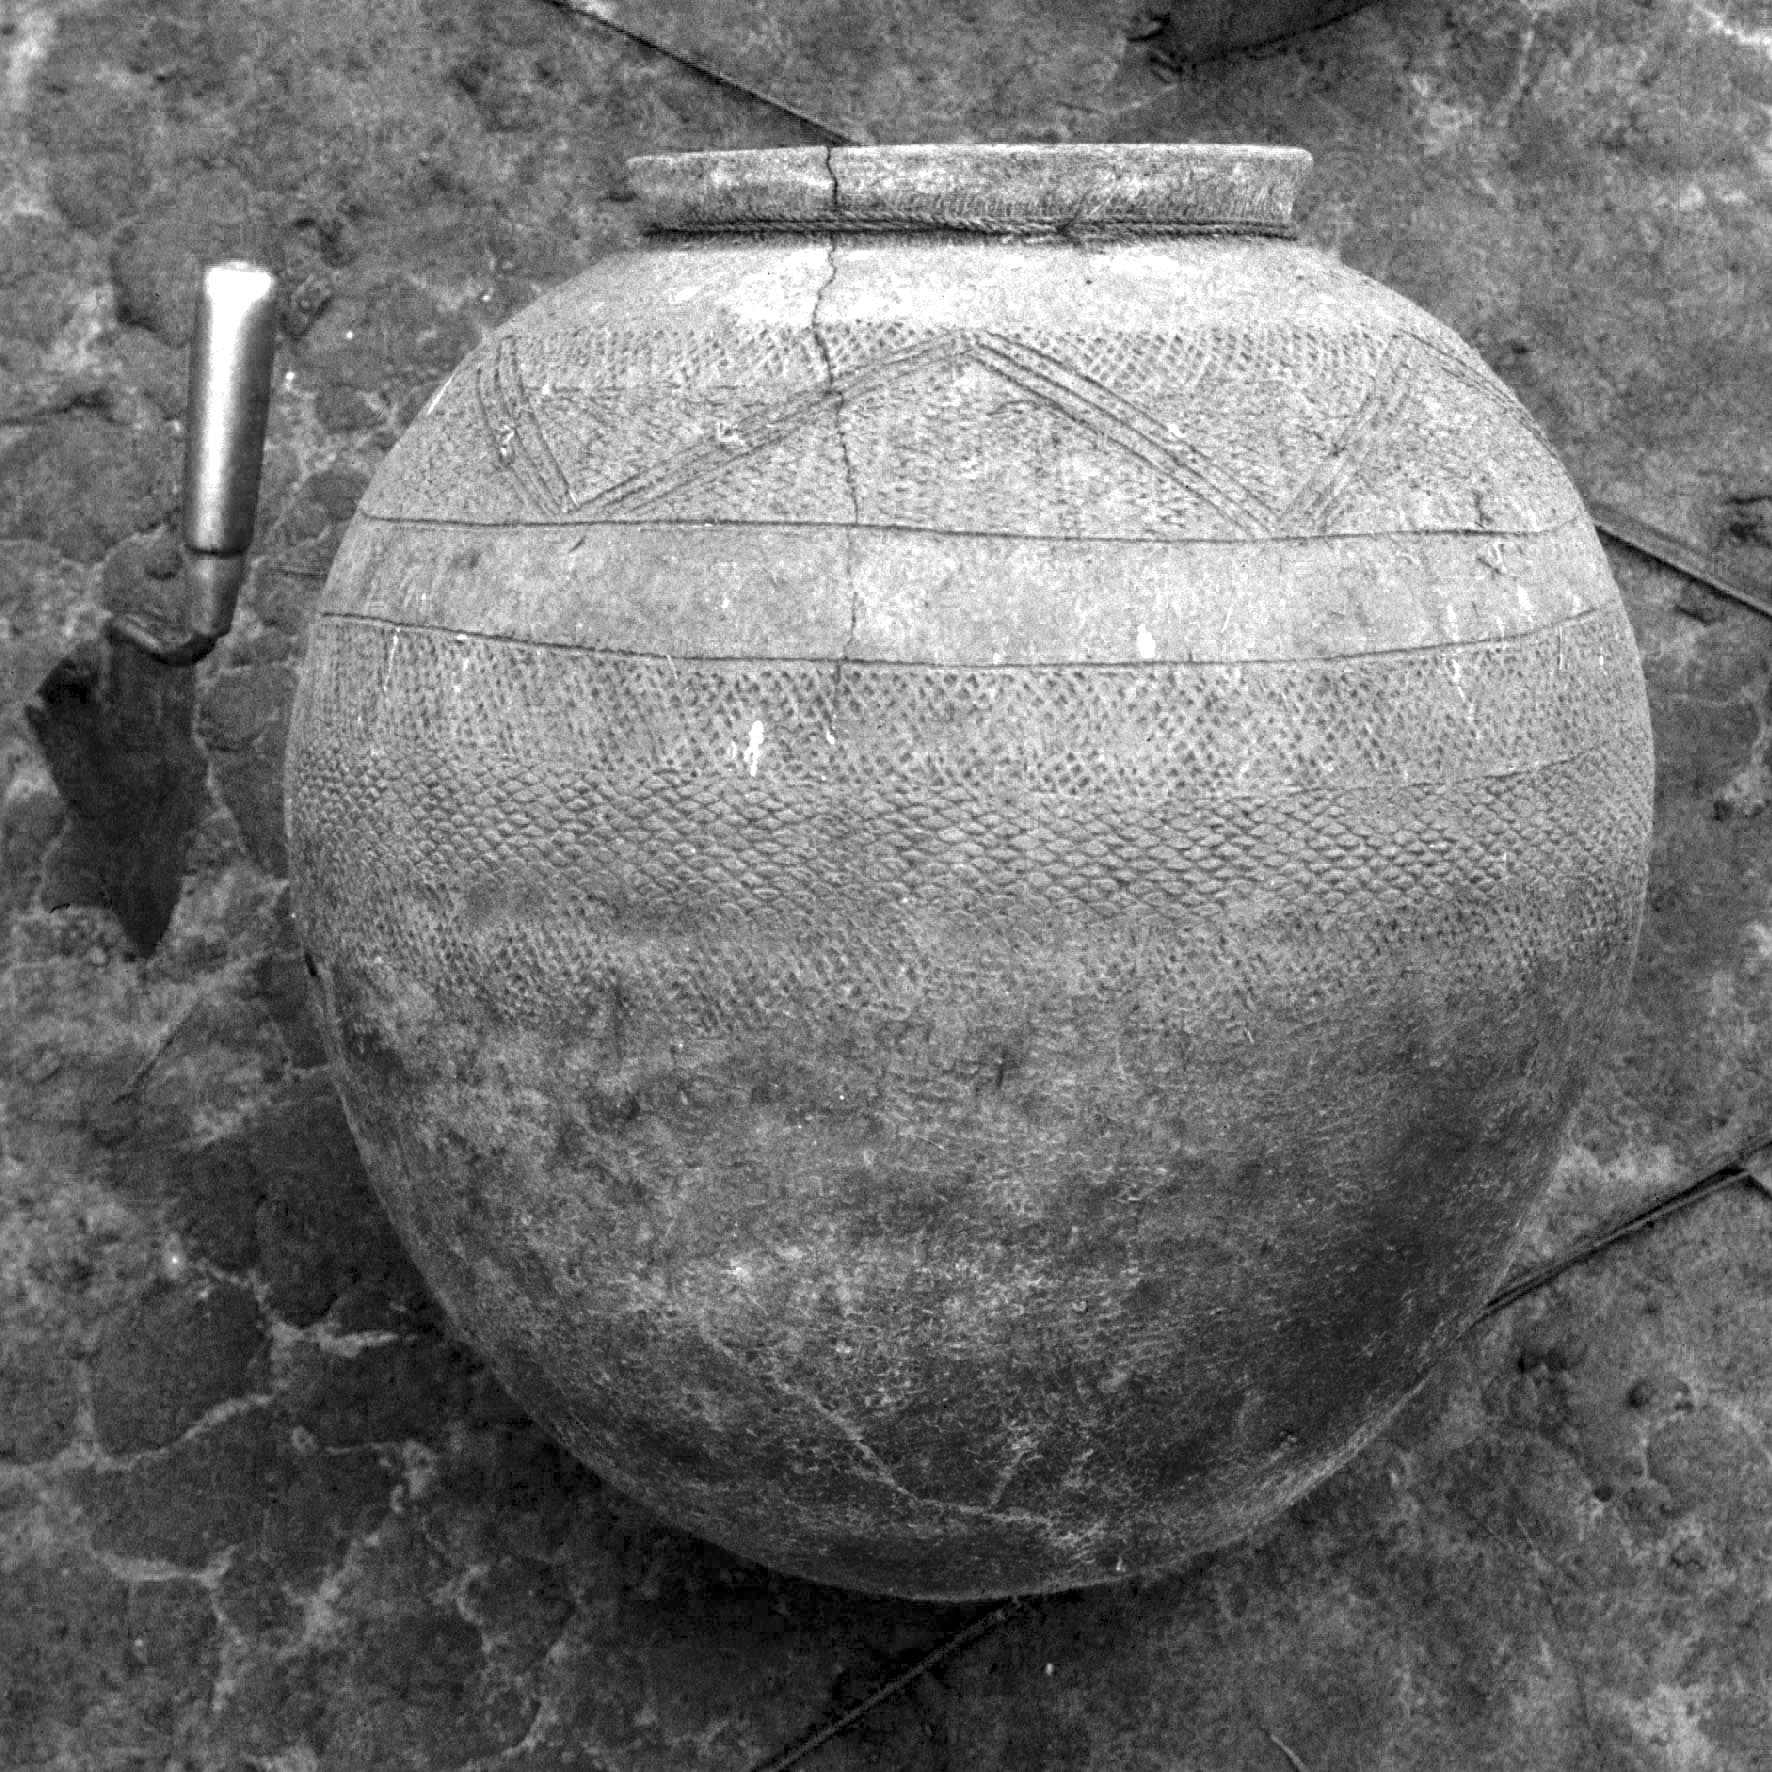
\includegraphics[width=\textwidth]{figs/KPT85-101_Gef_E85-024-9.jpg}
		\caption{Gefäß mit konvexer Wandung und kurzem, ausbiegendem Rand (Foto: M. K. H. Eggert).}
		\label{fig:KPT85_Foto-Gef}
	\end{subfigure}
	\begin{subfigure}[b]{.49\textwidth}
		\centering
		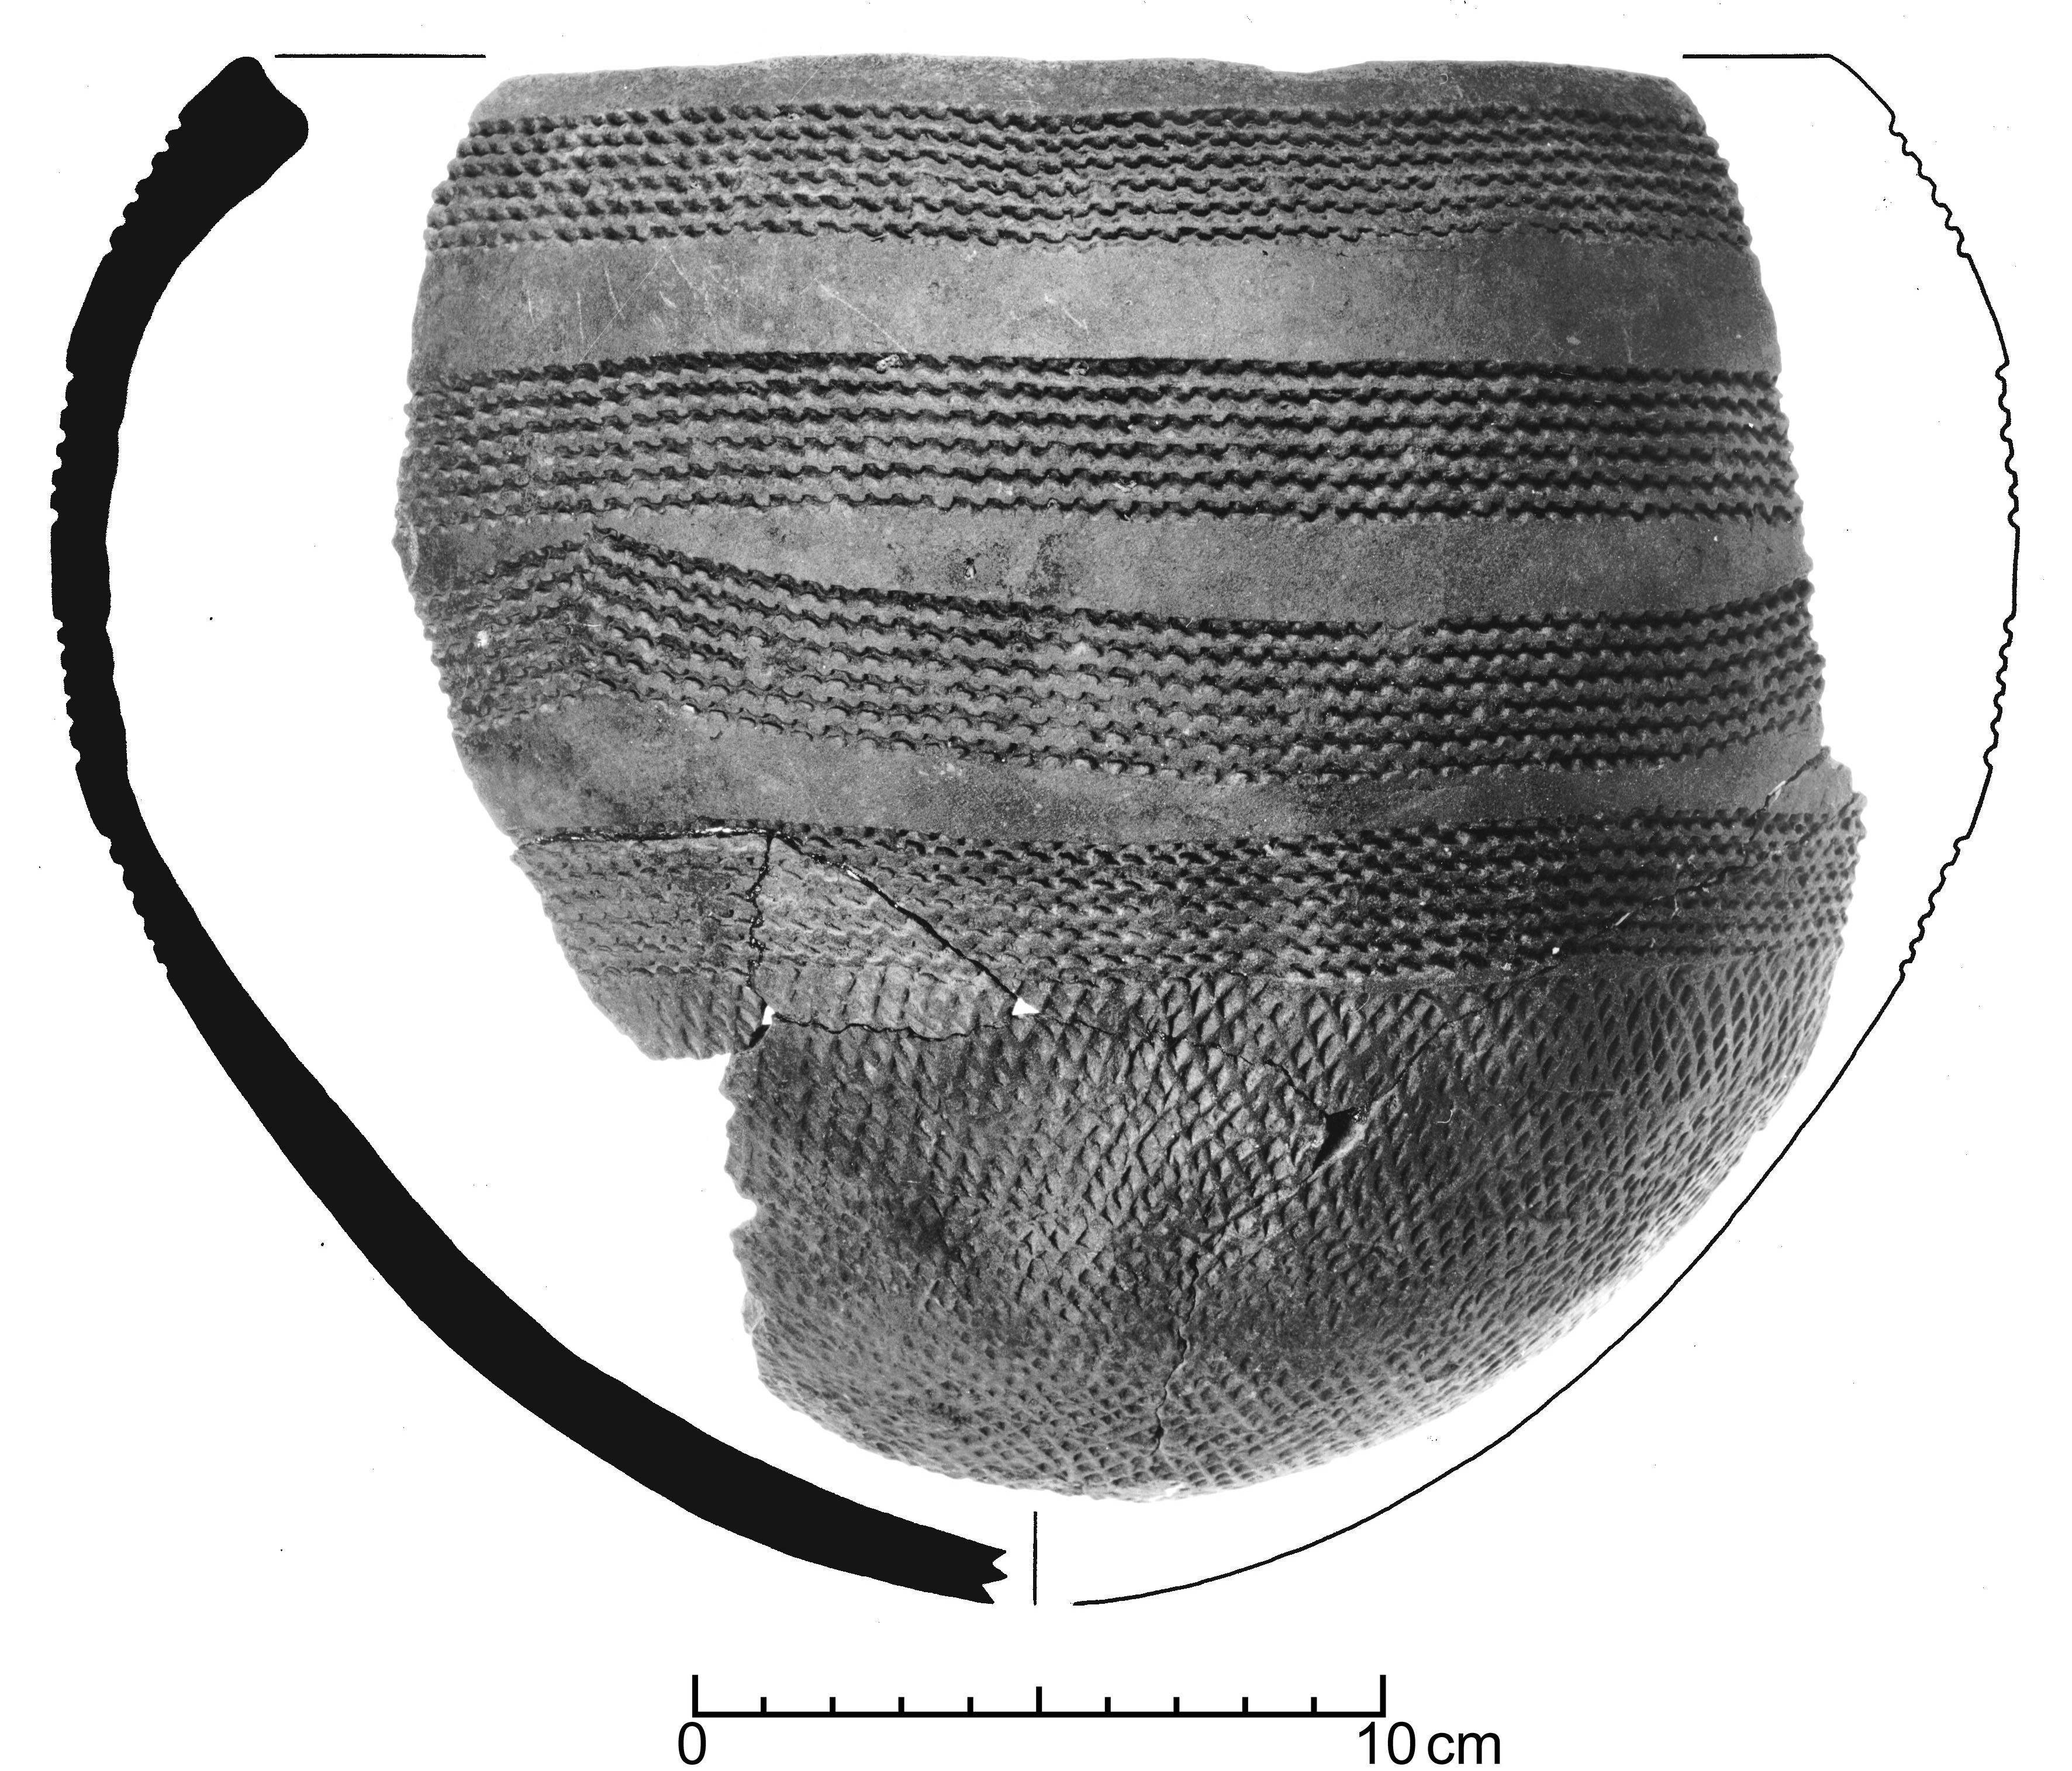
\includegraphics[width=.95\textwidth]{figs/KPT85-101-10_M1-2_M.jpg}
		\caption{Schalenförmiges Gefäß mit konvexer Wandung und einbiegendem Rand (H1; Taf.~22.1).}
		\label{fig:KPT85-101-Gef}
	\end{subfigure}
	\caption{Kpetene (Fpl.~220): Gefäße der Kpetene-Gruppe.}
	\label{fig:KPT85_Typvertreter}
\end{figure*}

\paragraph{Formen}
$\;$ \\
Die Hälfte aller der Kpetene-Gruppe zugewiesenen GE sind rund- bis spitzbodige hohe schalenförmige Gefäße mit einbiegenden Rändern (H1; Abb.~\ref{fig:KPT85-101-Gef}). Bei zwei weiteren GE blieb unklar, ob es sich um eine eher flache Variante der gleichen Grundform handelt (H2). Eine Ausnahme bildet ein am eponymen Fundplatz Kpetene fotografiertes Gefäß (Abb.~\ref{fig:KPT85_Foto-Gef}). Es handelt sich um ein rundbodiges, stark bauchiges Gefäß ohne ausgeformten Halsbereich, das über einen kurzen, leicht ausbiegenden Rand verfügt (D2). Gemein mit den anderen GE der Kpetene-Gruppe hat es die langovale Grundform mit rundem Boden sowie seine aus mehreren Bändern bestehende Rouletteverzierung.

Die rund- bis spitz-bodigen Schalen der Kpetene-Gruppen zeigen regelmäßig einbiegende Ränder (C3; Abb.~\ref{fig:KPT85-101-Gef}). Lediglich das fotografierte Gefäß verfügt über einen kurzen, ausbiegenden Rand (B1; Abb.~\ref{fig:KPT85_Foto-Gef}). Die Mündungen sind regelmäßig schräg nach innen abgestrichen (M6). Zwei GE weisen gerillte Randlippen auf (M4).

\begin{figure*}[p]
	\centering
	\includegraphics[width=\textwidth]{GIS/output/3-1-1-8_KPT_Verbreitung.pdf}
	\caption{Kpetene-Gruppe: Verbreitung.}
	\label{fig:KPT_Verbreitung}
\end{figure*}

\paragraph{Verzierungen}
$\;$ \\
Durch die Nutzung verschiedener Verzierungselemente werden die GE der Kpetene-Gruppe regelhaft in einen unteren sowie einen oberen Teil untergliedert. Während der untere Teil flächigen Mattenabdruck (Tab.~\ref{tab:Verzierungselemente}: 12) zeigt, zeichnet sich der obere Teil durch horizontale, alternierende Bänder mit Schnitzroulette aus (Abb.~\ref{fig:KPT85_Typvertreter}). Die gebänderte Verzierung der Gefäßoberteile kann neben verschiedenen Schnitzroulette-Variationen auch Ritzverzierungen umfassen (Abb.~\ref{fig:KPT85_Foto-Gef}). Eine GE weist drei mit dem gleichen Roulette gefertigte horizontale  Bänder sowie ein bogenförmiges, girlandenartiges Band auf (Abb.~\ref{fig:KPT85-101-Gef}). Der bestimmende Anteil der Verzierungselemente der Kpetene-Gruppe sind verschiedene Variationen von Schnitzroulette (Tab.~\ref{tab:Verzierungselemente}: 21.5, 21.7 und 21.12).

Eine großer Teil der Verzierungselemente der Kpetene-Keramik machen verschiedene Formen von Schnitzrouletteverzierung aus (58\,\%). Vegetabilische Roulette wurde in keinem Fall beobachtet. Das Schnitzroulette findet sich ohne Ausnahme auf den oberen Gefäßteilen, auf dem Bauch sowie im Schulterbereich der Gefäße. Nur eine GE zeigt auch Schnitzroulette auf dem Rand. In seltenerem Maße treten auch horizontale Rillen auf (Tab.~\ref{tab:Verzierungselemente}: 02.1; 15\,\%). Sehr viel seltener lassen sich im Material horizontale Bänder aus feinen Eindrücken beobachten (Tab.~\ref{tab:Verzierungselemente}: 04.16; 8\,\%; Abb.~\ref{fig:KPT85-101-Gef}). Lediglich bei einer GE konnte die Form des Bodens beobachtete werden. Es handelte sich um einen leicht spitzen Rundboden. Die fotografierte GE aus Kpetene zeigt ebenfalls einen runden, leicht spitz zulaufenden Boden (Abb.~\ref{fig:KPT85_Foto-Gef}).

\paragraph{Datierung}
$\;$ \\
Für die Keramik der Kpetene-Gruppe liegen keine absoluten Datierungen vor. Jedoch unterstreicht die Beobachtung eines noch in Benutzung befindlichen Gefäßes am eponymen Fundplatz Kpetene (Fpl. 220) am oberen Ubangi zum Zeitpunkt der Befahrung im Jahr 1985 den rezenten Charakter des entsprechenden Materials (Abb.~\ref{fig:KPT85_Foto-Gef}). Mit Blick auf die Schnitzroulette-Bänder zeigt das Material gewisse Ähnlichkeiten zu jener Keramik, die in Nana-Modé, in der Zentralafrikanischen Republik ausgegraben wurde \parencite{David.1977}. Auch dieses Material zeigt horizontale sowie girlandenartige Schnitzroulettebänder (ebd. 34 Abb.~7,1,3--6). Das Material der Kpetene-Gruppe setzt sich von der rezenten, Schnitzrouletteverzierten Keramik der Dama-Gruppe (Kap.~\ref{sec:DAM-Gr}) sowohl durch seine ornamentalen, flächige anstatt lediglich einzelne Bänder im Schulterbereich, als auch seine morphologischen Eigenheiten, spitzbodige hohe  Gefäßtypen, ab. Von der ebenfalls rezenten Mbati-Ngombe-Keramik (Kap.~\ref{sec:MBN-Gr}), die ähnliche Gefäßformen zeigt, unterscheidet sie sich durch die Verwendung von Schnitz- anstatt vegetabilischem Roulette.

\paragraph{Verbreitung}
$\;$ \\
Das Material der Kpetene-Gruppe wurde an fünf Fundplätzen entlang dem oberen Ubangi, stromauf von Bangui gefunden (Abb.~\ref{fig:KPT_Verbreitung}). Zweifelsfrei zuweisbare Stücke fanden sich lediglich in der namensgebenden Fundstelle Kpetene (Fpl.~220) und in Gbandami (Fpl.~226) sowie in Kouango (Fpl.~229). 